\chapter{Iteracion 6: Implementacion de un sistema gestionador para la placa de instrumentacion} % (fold)
\label{cha:iteracion_7}

\section{Introduccion} % (fold)
\label{it7:sec:introduccion}

Hasta el momento, utilizamos una computadora de uso comun para que configure el sistema y haga uso de sus funcionalidades. Pero, uno de los objetivos del proyecto es que sea un sistema embebido de un uso mas especifico el que realice estas acciones a la plataforma. Con esto en mente, consideramos que es necesario comprobar el funcionamiento del sistema con algun embebido que tome la funcion de recibir los datos de telemetria y controlar la plataforma.

La implementacion de este sistema embebido estara orientada al uso y control de la plataforma, y en particular, al control del sensor de campo electrostatico con el que se trabajo en la iteracion anterior. De esta forma, obtendremos una prueba de campo similar a un producto final.

El obejtivo principal es correr un programa en un sistema embebido, que se comunique con la plataforma de instrumentacion, sea capaz de configurarla, y tener acceso directo a las funcionalidades ligadas al sensor de campo electrostatico.

El programa sera desarrollada basandonos en partes del proyecto integrador de Gaston Lucero. El proyecto de Lucero consiste en un sistema gestionador de dispositivos IoI. Parte del software de gestion es un servidor web desarrollado en python, que es posible de embeber en una placa de desarrollo y actuar como el sistema gestionador al que se le envian los datos de telemetria. En esta iteracion, trabajaremos sobre este software, intentando adaptarlo al uso con nuestra plataforma, con el fin de cumplir con los objetivos de la iteracion.

% section introduccion (end)

\section{Requerimientos de la iteracion} % (fold)
\label{it7:sec:requerimientos_de_la_iteracion}

\begin{itemize}
\item Se deberia poder conectar el sistema de gestion a la placa de instrumentacion mediante protocolo serial UART.
\item Deberia estar en el mismo lugar fisico que la placa de alimentacion.
\item Deberia implementar un servidor web con una interfaz grafica de usuario.
\item Deberia permitir la misma configuracion que se le permite a un usuario que esta conectado directamente a la placa de instrumentacion, via una interfaz web grafica con conexion a internet. 
\item Deberia permitir establecer intervalos de fecha, hora y minuto para medir campo electrostatico en modo diferencial y en el pin 0 de la plataforma
\item Deberia guardar datos de mediciones e informacion sobre transacciones en general entre ambas placas en una base de datos local, accesible via la interfaz web grafica 
\item La conexion entre el sistema y el usuario (dispositivo del usuario: computadora con conexion a internet, smartphone) deberia ser via Wi-Fi o algun otro protocolo inalambrico
\end{itemize}

% section requerimientos_de_la_iteracion (end)


\section{Placa de desarrollo elegida para la implementacion} % (fold)
\label{it7:sec:placa_de_desarrollo_elegida_para_la_implementacion}

Teniendo en cuenta los requerimientos, listamos una serie de requisitos que debe cumplir la placa de desarrollo que se seleccione:

\begin{itemize}
  \item Deberia poder albergar un sistema operativo basado en Linux o Unix
  \item Deberia permitir la conexion de un adaptador Wi-Fi USB
  \item Deberia tener interfaz serial UART
\end{itemize}

Por cubrir con todos los requerimientos y por razones de disponibilidad, decidimos implementar este sistema en una placa de desarrollo Raspberry Pi B+ (figura \ref{fig:raspberrypi}), embebida con un sistema operativo Raspbian (Debian para Raspberry). Esta placa de desarrollo cumple con todos los requisitos mencionados anteriormente, por lo que es posible cubrir todos los requerimientos del sistema de gestion.

\begin{figure}[h]
  \centering
  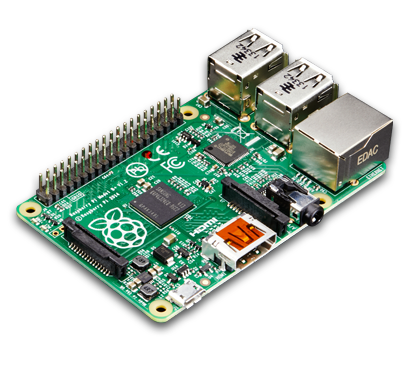
\includegraphics[width=0.80\textwidth, height = 7cm]{raspberrypi.png}
  \caption{Placa de desarrollo Raspberry Pi B+}\label{fig:raspberrypi}
\end{figure}
% section placa_de_desarrollo_elegida_para_la_implementacion (end)

\section{Diagramas de bloques} % (fold)
\label{it7:sec:diagramas_de_bloques}

Como etapa inicial del desarrollo, procedemos a graficar diagramas de bloques que describen el diseño estatico del sistema.

\begin{figure}[h]
  \centering
  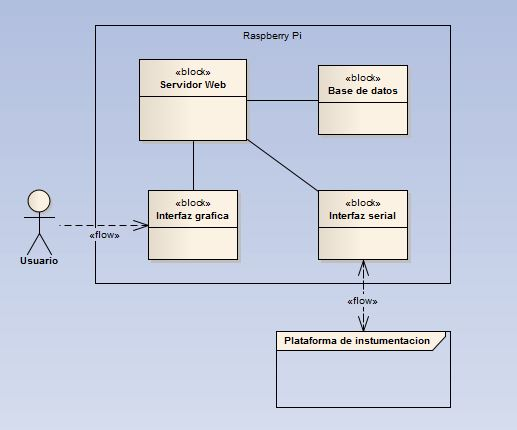
\includegraphics[width=0.80\textwidth, height = 7cm]{bloquessistemadegestion}
  \caption{Diagrama de bloques del sistema de gestion, implementado en una placa de desarrollo Raspberry Pi.}\label{fig:bloquessistemadegestion}
\end{figure}

\begin{figure}[h]
  \centering
  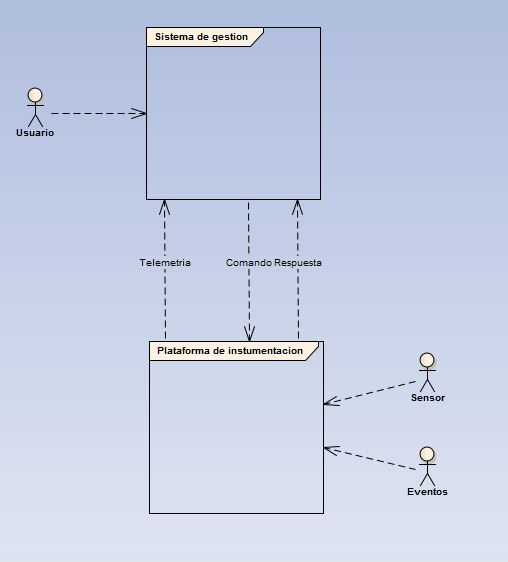
\includegraphics[width=0.80\textwidth, height = 7cm]{interaccionplataformaygestionador}
  \caption{Diagrama que ilustra la interaccion entre la plataforma de instrumentacion y el sistema gestionador}\label{fig:interaccionplataformaygestionador}
\end{figure}

La Figura \ref{fig:bloquessistemadegestion} muestra los distintos bloques del sistema de gestion y la figura \ref{fig:interaccionplataformaygestionador} ilustra la interaccion con la plataforma de instrumentacion. El sistema esta compuesto por cuatro bloques basicos:

\begin{itemize}
  \item Una interfaz grafica, que interactua con el usuario
  \item Una interfaz serial, que interactua con la plataforma de instrumentacion
  \item Un bloque que maneja el sistema de gestion de una base de datos MySQL, para guardar la informacion de telemetria junto con los metadatos
  \item Un Servidor Web, que ademas de proveer conexion a internet, maneja los bloques mencionados.
\end{itemize}


% section diagramas_de_bloques (end)

\section{Servidor web} % (fold)
\label{it7:sec:servidor_web}

El servidor web fue desarrollado con ayuda de BottlePy. BottlePy es un Web Framework liviano, simple y rapido, sin otra dependencia que la libreria estandar de Python. Incluye un servidor web HTTP, soporta mapeo de funciones a direcciones URL, y tiene un motor de generacion de documentos HTML en base a templates programadas en Python.

Con el uso de este servidor, disponemos una conexion al servidor en una direccion IP fija dentro de una red LAN. Con un modulo Wi-Fi USB conectado a la placa Raspberry Pi, es posible tener conexion a una red LAN. Si un usuario de la misma red se conecta al puerto 80 (HTTP) de esa direccion IP en un navegador, podra visualizar la interfaz grafica del servidor, y asi interactuar con el sistema de forma remota.

Al servidor web realizado por Lucero, tambien hecho con uso de BottlePy, se le realizo una adaptacion hacia nuestros requerimientos. Se agregaron, modificaron y eliminaron funciones dentro del servidor web para orientarlo hacia nuestros objetivos. En particular, el cambio mas significativo fue agregarle una base de datos en MySQL, modificar la interfaz grafica en HTML, y agregar la funcionalidad de los intervalos para mediciones con el sensor de campo electrostatico.

% section servidor_web (end)

\subsection{Base de datos} % (fold)
\label{it7:sub:base_de_datos}

La base de datos fue desarrollada utilizando la libreria ``MySQLdb'' de Python, especializada para uso de MySQL en servidores web.

Cuando se activa la conversion continua por medio del servidor, la base de datos guarda todos los datos entrantes y los clasifica segun el modo de medicion y el pin o los pines por donde se mide. Se guarda el valor de la medicion y una marca de tiempo con fecha, hora, minuto y segundo; realizada con ayuda de internet, y con la marca de tiempo relativa proveniente de la plataforma.

SCREENSHOT DE LA BASE DE DATOS EN ACCION

% subsection base_de_datos (end)

\subsection{Interfaz grafica de usuario} % (fold)
\label{it7:sub:interfaz_grafica_de_usuario}

La interfaz grafica proporciona al usuario un metodo mas amigable para la interaccion con la plataforma, ademas de proveer algunas funcionalidades extra.

SCREENSHOTS DE LA INTERFAZ GRAFICA PARA EL MOTOR.

Desde esta interfaz, el usuario puede:

\begin{itemize}
  \item Enviar cualquiera de los comandos que pueda interpretar la plataforma, con sus correspondientes argumentos
  \item Medir de manera inmediata el pin 0 en modo canal unico
  \item Encender/Apagar el motor del sensor de campo electrostatico
  \item Establecer uno o varios intervalos de medicion, con fecha y hora, donde el sensor de campo electrostatico debera encenderse, medir campo electrico, y enviar los datos a la Raspberry Pi.
\end{itemize}


% subsection interfaz_grafica_de_usuario (end)


\section{Pruebas} % (fold)
\label{it7:sec:pruebas}

\begin{table}[h]
\centering
\caption{Test de sistema 1}
\label{it7:tab:testsistema1}
\begin{tabular}{p{2cm} p{9cm}}
\multicolumn{2}{c}{\cellcolor[HTML]{68CBD0}{\color[HTML]{000000} Prueba de sistema}} \\
Prueba \#        & 1 \\
\hline
Nombre           & Configuracion normal mediante la interfaz grafica \\                     
\hline
Requerimiento    & La interfaz grafica deberia permitir la misma configuracion que se le permite a un usuario que esta conectado directamente a la plataforma de instrumentacion.  \\
\hline
Descripcion      & Se intentaran realizar configuraciones normales de la plataforma, mediante el uso de la interfaz grafica del servidor web desarrollado \\
\hline
Pre-condiciones  & \tabitem Plataforma de instrumentacion encendida y disponible para configurar  \\
                 & \tabitem Sistema de gestion en la placa Raspberry Pi levantado y conectado a la red local a una direccion IP fija \\
                 & \tabitem Ordenador con navegador abierto conectado a la direccion IP de la Raspberry Pi. Deberia poder verse la interfaz grafica del servidor \\
                 & \tabitem Raspberry Pi conectada a la placa de instrumentacion mediante cable serial RS-232 \\
\hline

Post-condiciones & Los comandos deberian funcionar correctamente y de igual manera que si se ingresaran directamente en la plataforma de instrumentacion  \\
\hline
Secuencia  & Ingresamos el comando ``SSE,0,1'' en la interfaz grafica, y luego presionamos ``Enviar'' \\
\hline
Resultados       & La respuesta de la plataforma fue la respuesta exitosa del comando, indicando que se configuro el pin 0 en modo canal unico, con un intervalo de 1. \\
\end{tabular}
\end{table}


\begin{table}[h]
\centering
\caption{Test de sistema 2}
\label{it7:tab:testsistema2}
\begin{tabular}{p{2cm} p{9cm}}
\multicolumn{2}{c}{\cellcolor[HTML]{68CBD0}{\color[HTML]{000000} Prueba de sistema}} \\
Prueba \#        & 1 \\
\hline
Nombre           & Intervalos de medicion \\                     
\hline
Requerimiento    & Establecer intervalos de tiempo usando hora y fecha en los que se debe medir sobre algun canal, pudiendo elegir el modo y el intervalo del mismo.  \\
\hline
Descripcion      & Verificar la funcionalidad de los intervalos de medicion para el sensor de campo electrostatico \\
\hline
Pre-condiciones  & \tabitem Plataforma de instrumentacion encendida y disponible para configurar  \\
                 & \tabitem Sistema de gestion en la placa Raspberry Pi levantado y conectado a la red local a una direccion IP fija \\
                 & \tabitem Ordenador con navegador abierto conectado a la direccion IP de la Raspberry Pi. Deberia poder verse la interfaz grafica del servidor \\
                 & \tabitem Raspberry Pi conectada a la placa de instrumentacion mediante cable serial RS-232 \\
                 & \tabitem Circuito de adaptacion del sensor alimentado \\
                 & \tabitem Sensor apagado\\
\hline

Post-condiciones & El motor deberia encenderse, medir durante el tiempo que dure el intervalo, enviar los datos por protocolo serial a la Raspberry Pi, y apagarse cuando finalice el tiempo del intervalo   \\
\hline
Secuencia  & \tabitem a las 15:00 hs, establecimos un intervalo entre las 15:01 y las 15:05, dando un total de 4 minutos de medicion. \\
\hline
Resultados       & A las 15:01, se inicio la secuencia de arranque del motor, y luego de eso comenzo a enviar los datos de telemetria. Comprobamos que ningun eslabon fallaba al perturbar el campo electrico del sensor y verificar que los datos en la base de datos se correspondian con estas perturbaciones.
\end{tabular}
\end{table}

% section pruebas (end)

\section{Conclusiones} % (fold)
\label{it7:sec:conclusiones}

Desde un punto de vista conceptual, esta ultima iteracion fue realizada con el objetivo de generar abstraccion entre los distintos sistemas. El servidor web que se ejecuta en la Raspberry Pi tiene la funcion de traducir acciones sobre una interfaz, en comandos, sobre otra interfaz; ademas de otras funciones adicionales. La plataforma de instrumentacion fue diseñada de tal manera de permitir faclidad a la hora de diseñar un sistema de gestion que la controle. Los comandos y las respuestas son cadenas estructuradas de caracteres; esto amplia la cantidad de sistemas embebidos compatibles con nuestra plataforma. Asi, se verifica que se cumple con uno de los requerimientos no funcionales de la plataforma: Portabilidad.

Al finalizar esta iteracion, quedaron algunas partes sin concluir, en lo que respecta al servidor web en la Raspberry Pi. Pero, los requerimientos principales fueron cumplidos, a pesar de las limitaciones del servidor web desarrollado.
A pesar de esto, logramos obtener un prototipo de producto que puede ser considerado como un detector inteligente de campo electrostatico. Partiendo de la plataforma de instrumentacion, junto con el sensor y el servidor web en la Raspberry Pi, es posible que este prototipo evolucione a convertirse en un producto real.


% section resultados (end)

% chapter iteracion_7 (end)